\section{釜式反应器中复合反应的收率与选择性}


\begin{frame}
    \frametitle{复合反应的收率与选择性的影响因素}

    \large 在反应器中进行复合反应时，目的产物的收率如何，是首先要考虑的事，因为它直接影响到产品的数量与质量；反应选择性也同样重要，它反映了原料利用的程度。
    
    \begin{itemize}
        \item[\bullet] 反应器的型式
        \item[\bullet] 反应器的操作方式
        \item[\bullet] 反应器的操作条件
    \end{itemize}
    下面将针对釜式反应器对这些影响因素进行分析讨论。

\end{frame}


\begin{frame}
    \frametitle{总收率与总选择性}

    设生成lmol目的产物P所需反应物A的量为$\mu_\mathrm{PA}$ mol，由第二章知，瞬时选择性为
    \[
        S=\mu_{\mathrm{PA}} \frac{\mathscr{R}_{\mathrm{p}}}{(-\mathscr{R}_{\mathrm{A}})}=\mu_{\mathrm{PA}} \frac{\mathrm{d} n_{\mathrm{p}}}{(-\mathrm{d} n_{\mathrm{A}})}=\frac{\mathrm{d} Y_{\mathrm{p}}}{\mathrm{d} X_{\mathrm{A}}}
    \]
    由于$S$为瞬时值，显然$X_\mathrm{A}$和$Y_\mathrm{P}$也都是瞬时值。就间歇反应器而言三者均随时间而变；而对于定态下操作的流动反应器，三者均随位置而改变（连续釜式反应器例外）。如果将上式改写成$\mathrm{d}Y_\mathrm{P}=S\mathrm{d}X_\mathrm{A}$并积分之得
    \[
        Y_{\mathrm{Pf}}=\int_{0}^{X_{\mathrm{Af}}} S \mathrm{~d} X_{\mathrm{A}}
    \]
    此时$Y_{\mathrm{Pf}}$称为总收率或最终收率，$X_{\mathrm{Af}}$为总转化率或最终转化率，两者不再是瞬时值，而是反应过程的总结果，即$Y_{\mathrm{Pf}}$和$X_{\mathrm{Af}}$系对整个反应器而言的值。
\end{frame}


\begin{frame}
    \frametitle{总收率与总选择性}

    由转化率、收率和选择性的定义得
    \[
        Y_{\mathrm{Pf}}=S_\mathrm{O}X_{\mathrm{Af}}
    \]
    $S_\mathrm{O}$叫做总选择性，是就整个反应器而言的选择性，是一个积分值，所以又叫做积分选择性。

    总选择性与瞬时选择性的关系为
    \[
        S_\mathrm{O}=\frac{1}{X_{\mathrm{Af}}}\int_0^{X_{\mathrm{Af}}}S\mathrm{d}X_{\mathrm{A}}
    \]
    总选择性与转化率的关系取决于反应动力学、反应器型式和操作方式等，一般为一个很复杂的关系式。所以，同样是釜式反应器，由于操作方式不同，虽然最终转化率一样，但最终收率却是不一样的。

\end{frame}


\begin{frame}
    \frametitle{釜式反应器的最终收率}
    \begin{figure}[htpb]
        \centering
        
\includegraphics[width=.9\linewidth]{fig3.9}
    \end{figure}

    (a)情况，相同最终转化率下，收率大小：间歇釜>多釜串联>单个连续釜

    (b)情况，相同最终转化率下，收率大小：间歇釜<多釜串联<单个连续釜
\end{frame}


\begin{frame}
    \frametitle{平行反应}

    设在釜式反应器中进行如下平行反应
    \[
        \mathrm{A}+\mathrm{B} \longrightarrow \mathrm{P} \qquad r_{\mathrm{p}}=k_{1} c_{\mathrm{A}}^{\alpha_{1}} c_{\mathrm{B}}^{\beta_{1}} 
    \]
    \[
        \mathrm{~A}+\mathrm{B} \longrightarrow \mathrm{Q} \qquad r_{\mathrm{Q}}=k_{2} c_{\mathrm{A}}^{\alpha_{2}} c_{\mathrm{B}}^{\beta_{2}}
    \]    
    目的产物为P，瞬时选择性为
    \[
        S=\frac{1}{1+\frac{k_{2}}{k_{1}} c_{\mathrm{A}}^{\alpha_{2}-\alpha_{1}} c_{\mathrm{B}}^{\beta_{2}-\beta_{1}}}
    \]
    由此可见反应物系的浓度和温度是影响瞬时选择性的直接因素。比较主、副反应的反应级数，便可判定是在高浓度下操作还是在低浓度下操作有利，抑或是一个反应物浓度高而另一个低更为有利。温度条件则看主、副反应活化能的相对大小。设计反应器时就应尽可能满足这些有利的浓度和温度条件，以获得较好的产品收率。

\end{frame}


\begin{frame}{浓度对平行反应瞬时选择性的影响(第2章)}
	$$S=\frac{k_1c_\mathrm{A}^\alpha}{k_1c_\mathrm{A}^\alpha+|{\nu_\mathrm{A}}|k_2c_\mathrm{A}^\beta}=\frac{1}{1+\frac{k_2}{k_1}|{\nu_\mathrm{A}}|c_\mathrm{A}^{\beta -\alpha}}$$
	\\若温度一定，则$k_1$和$k_2$为常数，反应物浓度$c_\mathrm{A}$改变时，瞬时选择性的变化与主副反应级数有关。
	\begin{itemize}
		\item[\bullet ]  当$\alpha = \beta$时，S与浓度无关，仅为温度的函数
		\item[\bullet ]  当$\alpha > \beta$时，反应物浓度提高，S增加，高浓度操作有利
		\item[\bullet ]  当$\alpha < \beta$时，反应物浓度提高，S减小，低浓度操作有利
	\end{itemize}
\end{frame}


\begin{frame}
    \frametitle{釜式反应器的操作方式与加料方式}
    ~\\
    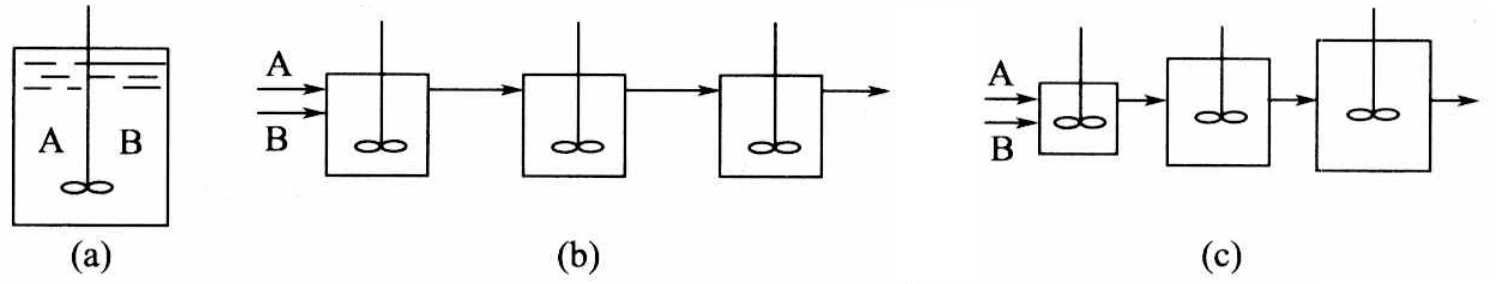
\includegraphics[width=\linewidth]{figs/fig3.10abc.png}
    \begin{itemize}
        \item[(a)] 如要求A和B的浓度都高，采用间歇操作是有利的
        \item[(b)] 如采用连续操作，则多釜串联为好，且组分A及B均从第一釜同时加入
        \item[(c)] 如采用不等体积的釜串联，体积依次增大会好些，因为这可使前两釜在更高一点的浓度下操作
    \end{itemize}
\end{frame}


\begin{frame}
    \frametitle{釜式反应器的操作方式与加料方式}
    $$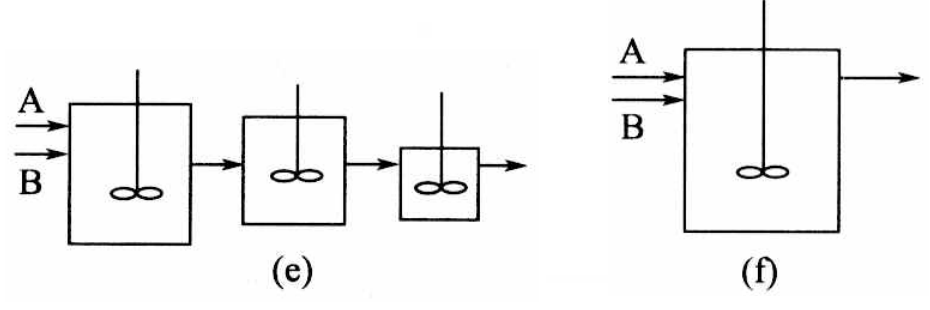
\includegraphics[width=0.8\linewidth]{figs/fig3.10ef.png}$$
    \begin{itemize}
        \item[(f)] 如要求A和B的浓度都低，采用单釜连续操作有利
        \item[(e)] 如采用多釜串联，则应做成不等体积的釜，且各釜体积依次减小，这样经过第一釜后反应物的浓度就可降得很低。
    \end{itemize}
\end{frame}


\begin{frame}
    \frametitle{釜式反应器的操作方式与加料方式}

    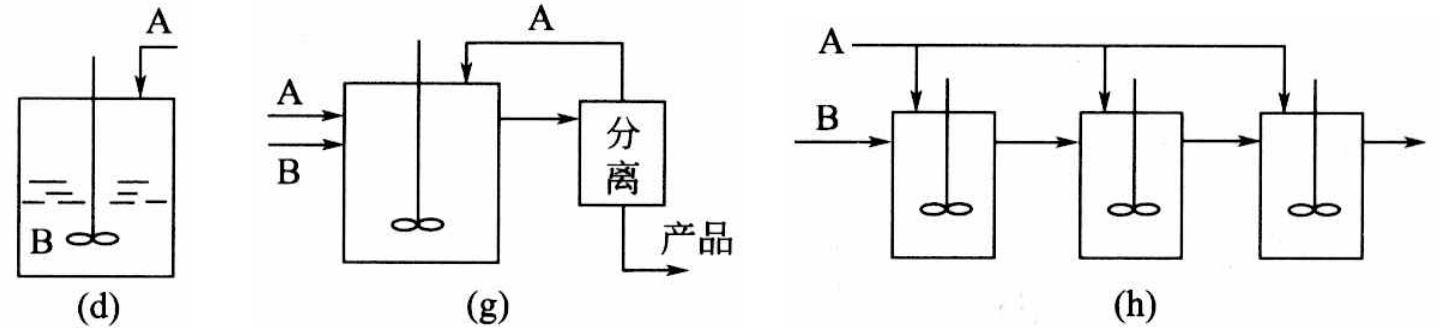
\includegraphics[width=\linewidth]{figs/fig3.10dgh.png}

    若要求一个组分浓度高另一组分浓度低，(d)(g)(h)均可选用。

    \begin{itemize}
        \item[(d)]  半间歇操作，B全部加入反应器内，A连续加入，加入速率一般由快变慢，这样可始终保持在A浓度低的情况下操作，而B的浓度则相对较大。
        \item[(h)]  连续操作，A分釜加入，结果可使A的浓度相应降低，而B的浓度则较高。
        \item[(g)] A过量配料，反应后产品分离，A和少量的B循环使用。A保持高浓度。
    \end{itemize}

\end{frame}


\begin{frame}[t]
    \frametitle{}
    \begin{example}
        以纯A为原料在连续釜式反应器中生产产物P，反应为
        \[
            \ch{A -> P} \qquad r_\mathrm{P} = k_1c_\mathrm{A}
        \]
        \[
            \ch{A -> U} \qquad r_\mathrm{U} = k_2c_\mathrm{A}
        \]
        反应速率常数$k_1$及$k_2$与温度的关系符合阿仑尼乌斯方程，指前因子$A_2 = 3.533\times 10^{18}$\ h$^{-1}$，$A_1 = 4.368\times 10^{15}$\ h$^{-1}$，反应活化能$E_1 = 41800$\ \si{J.mol^{-1}.K^{-1}}，$E_2 = 141000$\ \si{J.mol^{-1}.K^{-1}}。若空时为1 h，试问在什么温度下操作P的收率最大？
    \end{example}
\end{frame}


\begin{frame}
    \frametitle{连串反应(间歇釜)}
    在间歇釜式反应器中进行一级不可逆连串反应：$\mathrm{A} \stackrel{k_{1}}{\longrightarrow} \mathrm{P} \stackrel{k_{2}}{\longrightarrow} \mathrm{Q}$，
    在第3节已求得
    \[
        c_{\mathrm{P}}=\frac{k_{1} c_{\mathrm{A} 0}}{k_{1}-k_{2}}\left(e^{-k_{2} t}-e^{-k_{1} t}\right)
    \]
    将$t_{\mathrm{opt}}=\frac{\ln (k_{1} / k_{2})}{k_{1}-k_{2}}$代入得P的最大收率
    \[
        (Y_{\mathrm{P}, \mathrm{B}})_{\max }=(k_1/k_2)^{k_2/{(k_2-k_1)}} \qquad (k_1 \neq k_2)
    \]
    \[
        (Y_{\mathrm{P}, \mathrm{B}})_{\max }=1/e=0.368 \qquad \qquad (k_1 = k_2)
    \]
    将$t=\frac{1}{k_1}\ln \frac{1}{1-X_\mathrm{A}}$代入$c_{\mathrm{P}}$表达式得转化率与收率的关系
    \[
        Y_{\mathrm{P}, \mathrm{B}}=\frac{k_{1}}{k_{1}-k_{2}}\left[(1-X_{\mathrm{A}})^{k_{2} / k_{1}}-(1-X_{\mathrm{A}})\right] \qquad (k_{1} \neq k_{2})
    \]
    \[
        Y_{\mathrm{P}, \mathrm{B}}=(X_\mathrm{A}-1)\ln (1-X_\mathrm{A}) \qquad \qquad \qquad \qquad  (k_{1} = k_{2})
    \]
\end{frame}


\begin{frame}
    \frametitle{连串反应(连续釜)}
    在连续釜式反应器中进行一级不可逆连串反应
    \[
        \mathrm{A} \stackrel{k_{1}}{\longrightarrow} \mathrm{P} \stackrel{k_{2}}{\longrightarrow} \mathrm{Q}
    \]
    A及P的物料衡算式分别为：
    \[
        V_{r}=\frac{Q_{0}(c_\mathrm{A0}-c_\mathrm{A})}{k_{1}c_\mathrm{A}}
    \]
    \[
        V_{\mathrm{r}}=\frac{Q_{0}c_{\mathrm{p}}}{k_{1}c_{\mathrm{A}}-k_{2}c_{\mathrm{p}}}
    \]
    解得
    \[
        \begin{aligned}
            c_{\mathrm{A}}&=c_{\mathrm{A}0}/(1+k_{1}\tau) \\
            c_\mathrm{P}&= \frac{k_1\tau c_{\mathrm{A}0}}{(1+k_1\tau)(1+k_2\tau)}
        \end{aligned}
    \]
\end{frame}


\begin{frame}
    \frametitle{连串反应(连续釜)}
    \vspace{-6pt}
    \[
        Y_\mathrm{P,M} = \frac{c_\mathrm{P}}{c_\mathrm{A0}}= \frac{k_1\tau}{(1+k_1\tau)(1+k_2\tau)}
    \]
    对$\tau$求导，并令$\dif Y_\mathrm{p}/\dif t = 0$，得最佳空时
    \[
        \tau_\mathrm{op} = \frac{1}{\sqrt{k_1k_2}}
    \]
    代回$Y_\mathrm{P,M}$表达式得P的最大收率
    \[
       (Y_{\mathrm{P}, \mathrm{M}})_{\max }=\frac{k_{1}}{(\sqrt{k_{1}}+\sqrt{k_{2}})^{2}}
    \]
    将$\tau = \frac{X_\mathrm{A}}{k_1(1-X_\mathrm{A})}$代入$Y_\mathrm{P,M}$表达式得转化率与收率的关系
    \[
        Y_{\mathrm{P}, \mathrm{M}}=\frac{k_{1} X_{\mathrm{A}}(1-X_{\mathrm{A}})}{k_{2} X_{\mathrm{A}}+k_{1}(1-X_{\mathrm{A}})}
    \]
\end{frame}


\begin{frame}
    \frametitle{连续釜和间歇釜的收率与转化率的比较}

    \begin{minipage}{0.48\linewidth}
        \begin{figure}[htpb]
            \centering
            
\includegraphics[width=\linewidth]{fig3.11}
        \end{figure}
    \end{minipage}\hfill
    \begin{minipage}{0.48\linewidth}
        \begin{itemize}
            \item[$\rhd$ ] 无论$k_2/k_1$为何值，相同转化率下，间歇釜式反应器P的最大收率总是大于连续釜
            \item[$\rhd$ ] $k_2/k_1$值越小，$Y_\mathrm{p}$差异越大
            \item[$\rhd$ ] 每一曲线都存在极大值
            \item[$\rhd$ ] ABC、DEF分别为间歇釜和连续釜最大收率的轨迹
            \item[$\rhd$ ] 收率总是随着$k_2/k_1$的减小而增大。如何减小$k_2/k_1$？
        \end{itemize}
    \end{minipage}
\end{frame}


\begin{frame}
    \frametitle{如何减小$k_2/k_1$？}
    \begin{enumerate}
      \item 选择适宜的操作温度
        \[
        \frac{k_2}{k_1}=\frac{A_2}{A_1}\exp\bigl(\frac{E_1-E_2}{RT}\bigr)
        \]
    \begin{itemize}
      \item 若 $E_1 > E_2$ ， 温度越高 ， 则比值 ${k_2}/{k_1}$ 越小 ， 因而收率越大 ；
      \item 若 $E_1 < E_2$ ， 温度越低 ， 则比值 ${k_2}/{k_1}$ 越小 ， 因而收率越大。
      \item 温度低必然导致反应速率下降，从而反应器的生产强度减小，所以要选择适宜的操作温度
      \item 若 $E_1 = E_2$， 温度的变化已不能改变${k_2}/{k_1}$ 值 ， 但实际上仍以采用较高的温度操作为佳。
    \end{itemize}
      \item 选择合适的催化剂
        \begin{itemize}
          \item 选择有利 P 的生成反应而不利 P 的转化反应的催化剂
        \end{itemize}
    \end{enumerate}
    
\end{frame}


\begin{frame}[t]
    \frametitle{}

    \begin{example}
        原料以0.5 \si{m^3/min}的流量连续通入反应体积为20\si{m^3}的全混流反应器，进行液相反应：
        \[
        \mathrm{A} \longrightarrow \mathrm{R} \qquad r_{\mathrm{A}}=k_{1} c_{\mathrm{A}}
        \]
        \[
        \mathrm{2R} \longrightarrow \mathrm{D} \qquad r_{\mathrm{D}}=k_{2} c_{\mathrm{R}}^2
        \]    
        原料中A的浓度等于\SI{0.1}{kmol/m^3}，反应温度下，$k_1=0·1$\si{min^{-1}}，$k_2=1.25$\si{L.mol^{-1}.min^{-1}}，试计算反应器出口处A的转化率及R的收率。
    \end{example}\pause
    \begin{columns}[c]
        \column{7.5cm}
        \large $\begin{array}{l}
        \frac{V_{r}}{Q_{0}}=\frac{C_{A 0} X_{A}}{k_{1} C_{A 0}(1-X_{A})}=\frac{X_{A}}{0.1(1-X_{A})}\\
    
        X_{A}=0.80\\
        
        C_{A}=C_{A 0}(1-X_{A})=0.02  \mathrm{kmol} / \mathrm{m}^{3}  
    \end{array}$
        \column{6cm}
        \large $\begin{array}{l}
            \frac{V_{r}}{Q_{0}}=\frac{C_{R}}{k_{1} C_{A}-2 k_{2} C_{R}^{2}}\\
        
            C_{R}= \SI{0.02372}{kmol/m^3}\\
        
            Y_{R}={C_{R}}/{C_{A 0}}=23.72\%
        \end{array}$
    \end{columns}

\end{frame}